% Intended LaTeX compiler: lualatex
\documentclass[10pt, svgnames]{beamer}
\usepackage{graphicx}
\usepackage{longtable}
\usepackage{wrapfig}
\usepackage{rotating}
\usepackage[normalem]{ulem}
\usepackage{amsmath}
\usepackage{amssymb}
\usepackage{capt-of}
\usepackage{hyperref}
\usetheme{metropolis}
\author{Sappinandana Akamphon}
\date{\today}
\title{Bearings}
\subtitle{ME 310: Mechanical Design}
\usepackage{booktabs}
\institute{Department of Mechanical Engineering, TSE}
\date{}
\AtBeginSection[]{\begin{frame}{Outline}\tableofcontents[currentsection]\end{frame}}
\hypersetup{
 pdfauthor={Sappinandana Akamphon},
 pdftitle={Bearings},
 pdfkeywords={},
 pdfsubject={},
 pdfcreator={Emacs 30.0.50 (Org mode 9.6)}, 
 pdflang={English}}
\begin{document}

\maketitle
\begin{frame}{Outline}
\tableofcontents
\end{frame}


\section{Overview of Bearings}
\label{sec:org9b43995}

\begin{frame}[label={sec:org0555bfa}]{What are bearings?}
\begin{itemize}
\item A feature that allows relative motions between components
\item Linear motions
\item Rotary motions
\end{itemize}
\end{frame}

\begin{frame}[label={sec:org1120274}]{Two types of bearings}
\begin{itemize}
\item Contact: sliding or rolling

\item Non-contact: fluid film or magnetic
\end{itemize}

\begin{center}
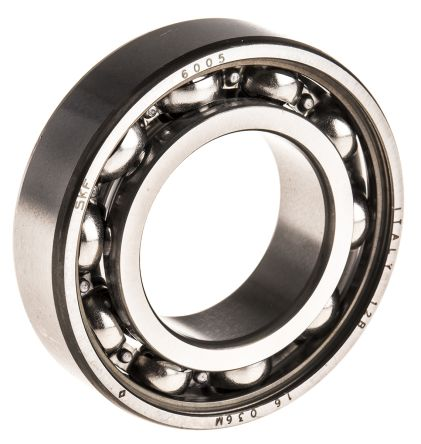
\includegraphics[width=0.45\textwidth]{./pictures/ball-bearing.jpg}
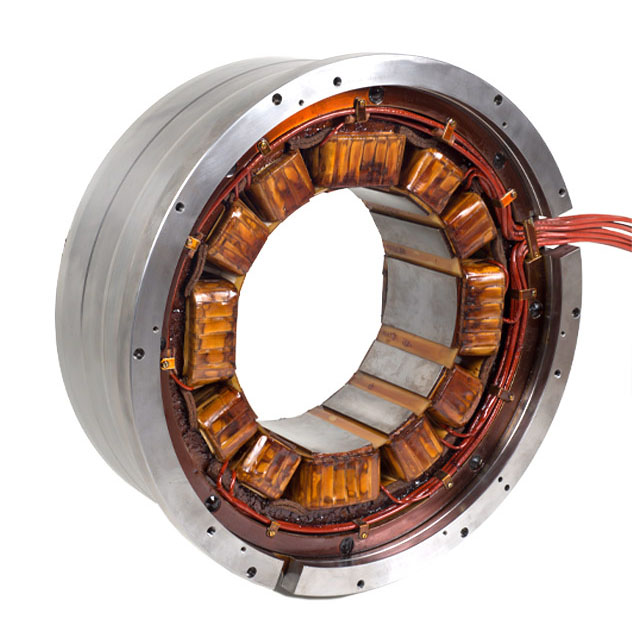
\includegraphics[width=0.45\textwidth]{./pictures/magnetic-bearing.jpg}
\end{center}
\end{frame}

\section{Sliding Contact Bearings}
\label{sec:orgf568ff4}

\begin{frame}[label={sec:org9c37f09}]{Sliding Contact Bearings}
\begin{itemize}
\item Commonly used in low- to medium-speed applications
\end{itemize}

\begin{center}
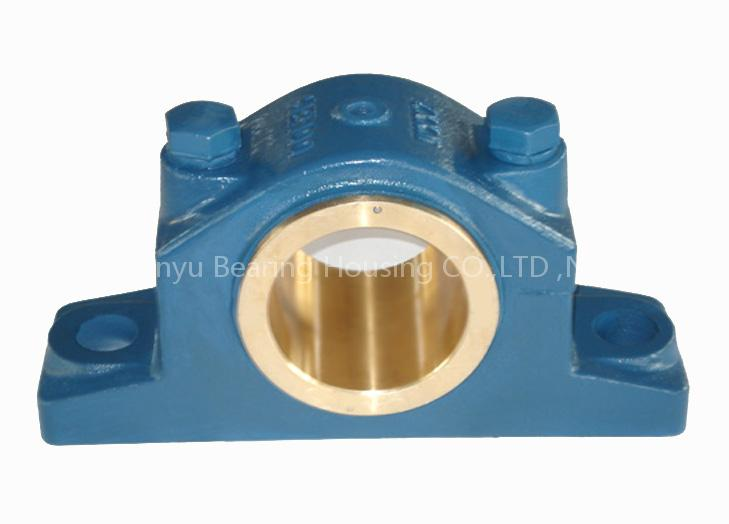
\includegraphics[width=0.7\textwidth]{./pictures/sliding-contact-bearing.jpg}
\end{center}

\begin{itemize}
\item Lubrication is used to reduce wear and friction
\end{itemize}
\end{frame}

\begin{frame}[label={sec:org2a937bc}]{Materials for Sliding Contact Bearing}
\begin{itemize}
\item Typically hard materials (shaft) on soft (bearing)
\item Materials:
\begin{itemize}
\item Polymers: nylon is king!
\item Brass
\item Ceramics
\end{itemize}
\item Check on bearing stress
\item Aluminum-on-aluminum is a no-no
\end{itemize}
\end{frame}

\begin{frame}[label={sec:org70154c5}]{Bearing Contact Pressure}
\begin{center}
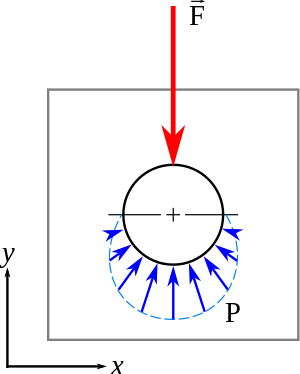
\includegraphics[height=0.6\textheight]{./pictures/elastic-cyl-on-cyl-pressure.png}
\end{center}

\begin{align*}
    P &= \frac{F}{DL} \\
    P_{\max} &= \frac{4}{\pi} \frac{F}{DL}
 \end{align*}
\end{frame}

\begin{frame}[label={sec:org8cb7d79}]{Sliding Contact Materials: PV Factor}
\begin{itemize}
\item (P)ressure \(\times\) (V)elocity
\item tradeoff in choosing bearing materials
\item higher pressure \(\rightarrow\) low speed, and vice versa
\end{itemize}
\end{frame}

\begin{frame}[label={sec:org4e9be24}]{PV Table for Metals}
\begin{center}
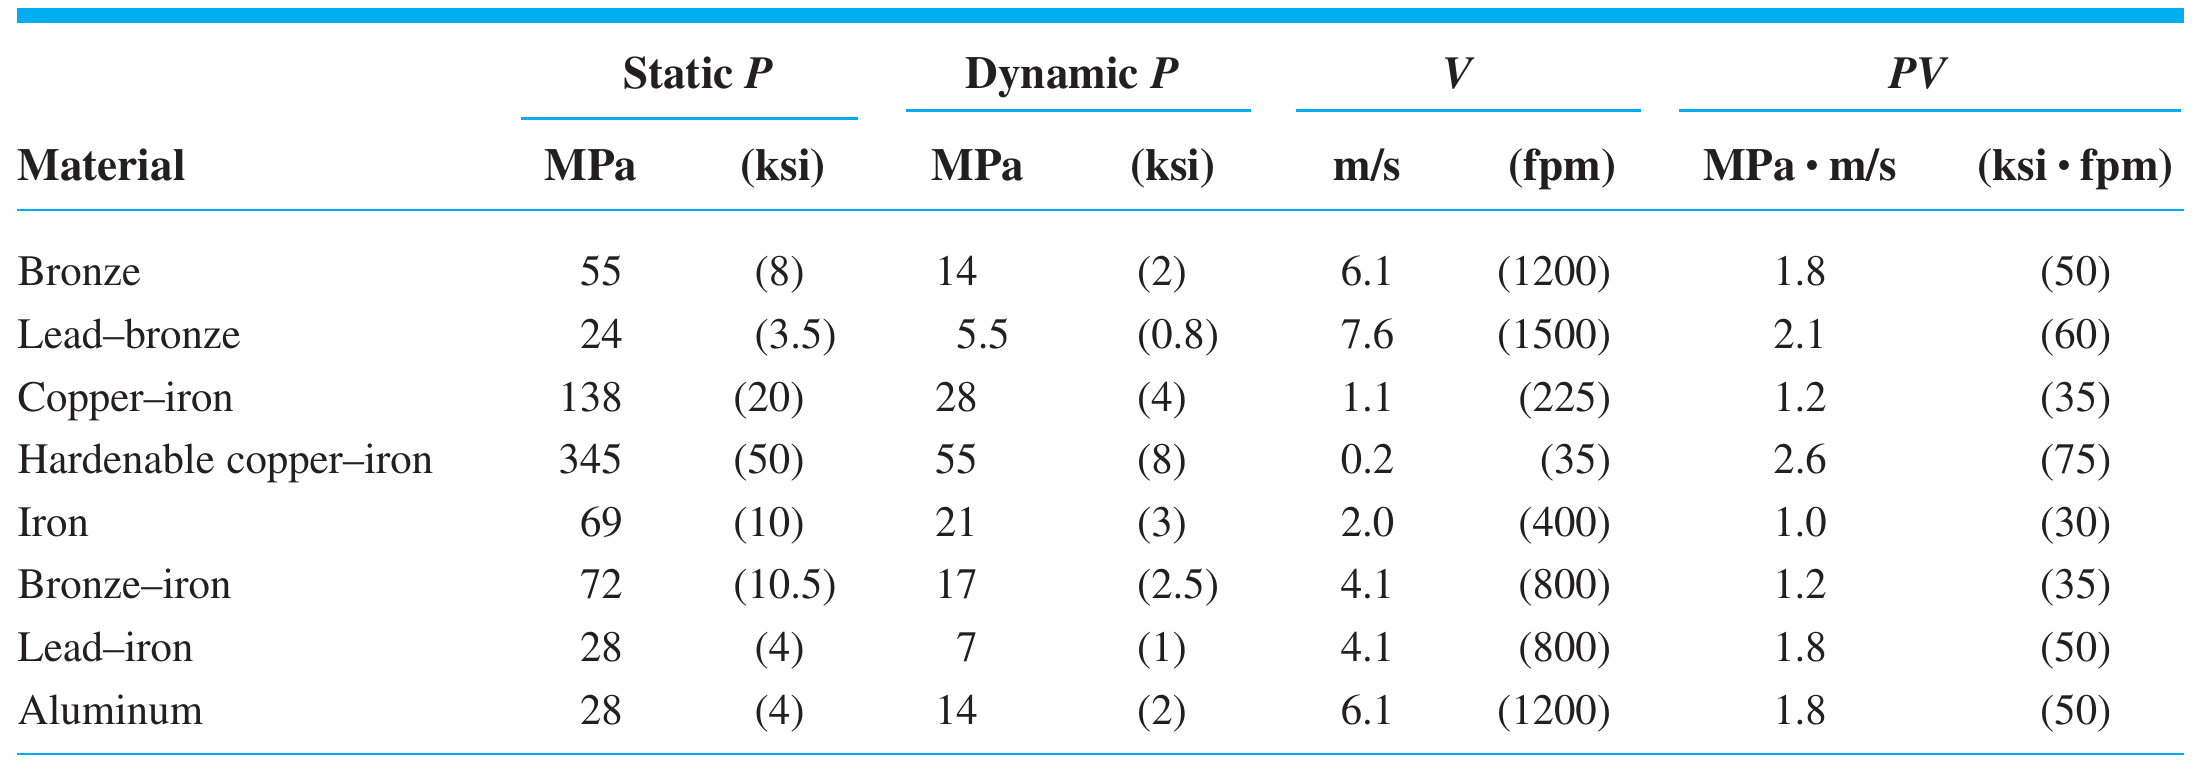
\includegraphics[width=\textwidth]{./pictures/pv-metal.png}
\end{center}
\end{frame}

\begin{frame}[label={sec:org71944fa}]{PV Table for Nonmetals}
\begin{center}
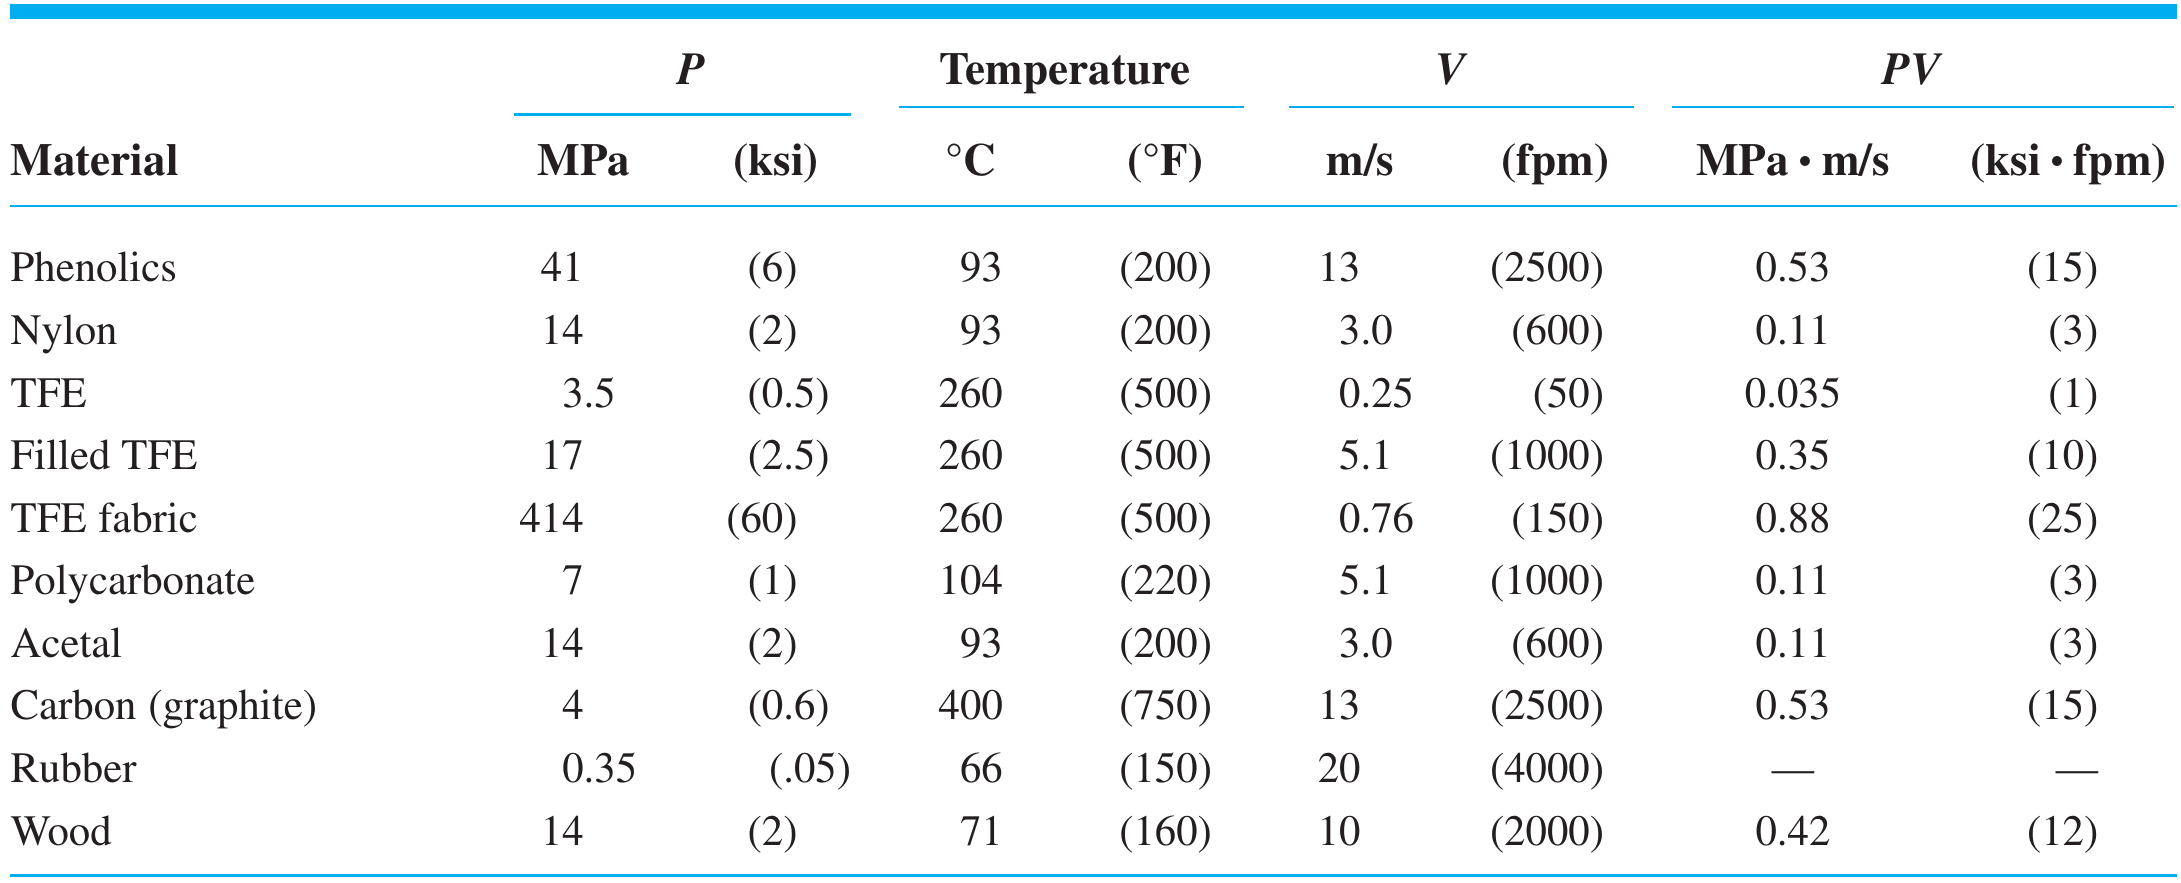
\includegraphics[width=\textwidth]{./pictures/pv-nonmetal.png}
\end{center}
\end{frame}

\begin{frame}[label={sec:orgeddfb66}]{Example: Sleeve Bearing for a Low-speed Shaft}
A 30-cm long shaft whose diameter \(D\) is 3 cm is operated at 1000 rpm. The shaft has a spur gear whose \(R_{\text{pitch}}\) = 10 cm mounted in the middle with a bearing at each end. The gear is transferring the power of 1.5 kW. The gear has pressure angle \(\theta\) = 20\(^{\circ}\). Determine the minimum bearing length \(L\) using nylon.
\end{frame}

\begin{frame}[label={sec:orgcdbdac8}]{Solution}
First, let us determine the force on the bearing. Since spur gears don't generate any axial load, the forces will simply be the radial + tangential load, perpendicular to the shaft.

\begin{align*}
    T &= \frac{P}{\omega} \\
      &= \frac{1500}{1000(2\pi / 60)} = 14.3 \text{ N-m} \\
    F &= \frac{T}{R_{\text{pitch}} \cos \theta} \\
      &= \frac{14.3}{0.1 \cos 20^{\circ}} = 152 \text{ N} \\
\end{align*}
\end{frame}

\begin{frame}[label={sec:org38faf86}]{Solution}
Since the gear is mounted in the middle, the force on each bearing is half of the force.

\begin{align*}
    F_{bearing} = \frac{152}{2} = 76 \text{ N}
\end{align*}

We can't determine the bearing pressure yet since we don't know the bearing length. We can determine the surface velocity, however.

\begin{align*}
    v = \omega (D/2) = 1000 (2\pi / 60) (0.03/2) = 1.57 \text{ m/s}
\end{align*}
\end{frame}

\begin{frame}[label={sec:orgd3f0d32}]{Solution}
We double-check that \(v < V_{nylon} (1.57 < 3.0)\) so nylon is an acceptable choice. The length of bearing, then should be

\begin{align*}
    P_{bearing}v &< (PV)_{nylon} \\
    \frac{F_{bearing}}{DL}v &< 0.11 \times 10^6 \\
    \frac{76}{0.03L} 1.57 &< 1.1 \times 10^5 \\
    L &> 0.036 = 3.6 \text{ cm}
\end{align*}
\end{frame}

\section{Rolling Contact Bearings}
\label{sec:org79d1178}

\begin{frame}[label={sec:org8ad564a}]{Rolling Elements}
\begin{itemize}
\item suitable for medium- to high-speed applications
\item use balls or rollers to avoid friction
\item load: roller \(>\) ball
\item friction: ball \(<\) roller
\end{itemize}
\end{frame}

\begin{frame}[label={sec:orge9dc45e}]{Rolling Element Types}
\begin{center}
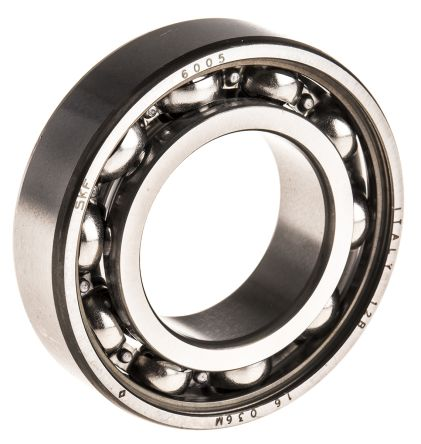
\includegraphics[width=0.3\textwidth]{./pictures/ball-bearing.jpg}
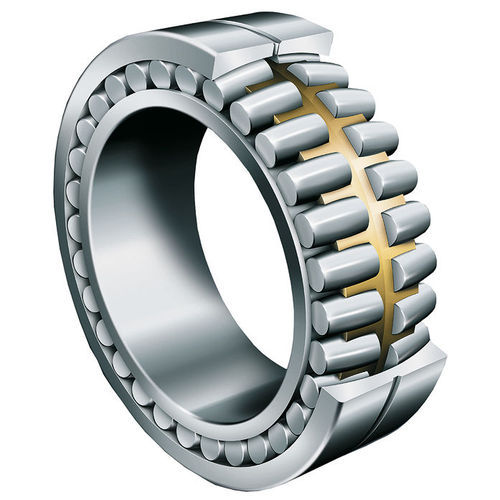
\includegraphics[width=0.3\textwidth]{./pictures/roller-bearing.jpg}
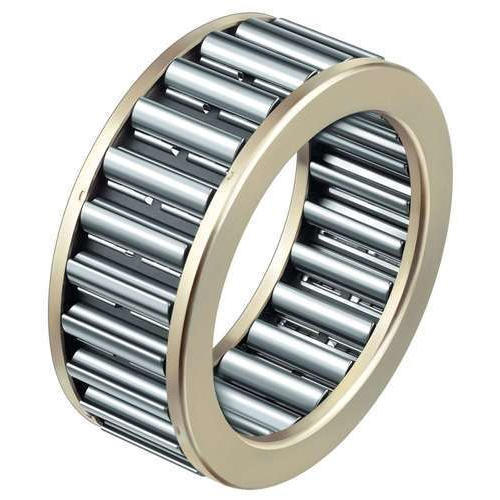
\includegraphics[width=0.3\textwidth]{./pictures/needle-roller-bearing.jpg}
\end{center}
\end{frame}

\begin{frame}[label={sec:org701db45}]{Radial vs Angular Contact Bearings}
\begin{center}
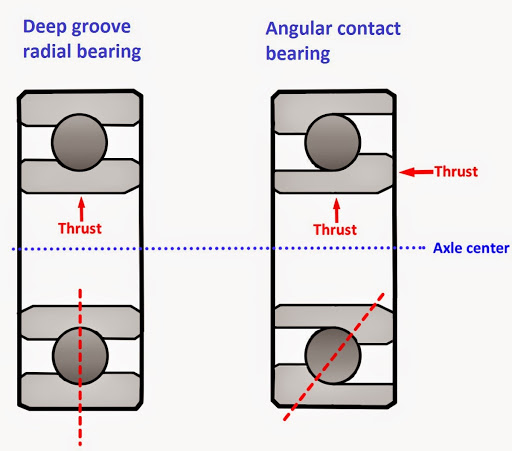
\includegraphics[width=.9\linewidth]{./pictures/radial-vs-angular.jpg}
\end{center}
\end{frame}

\begin{frame}[label={sec:org3bed9f2}]{Bearing Series}
\begin{center}
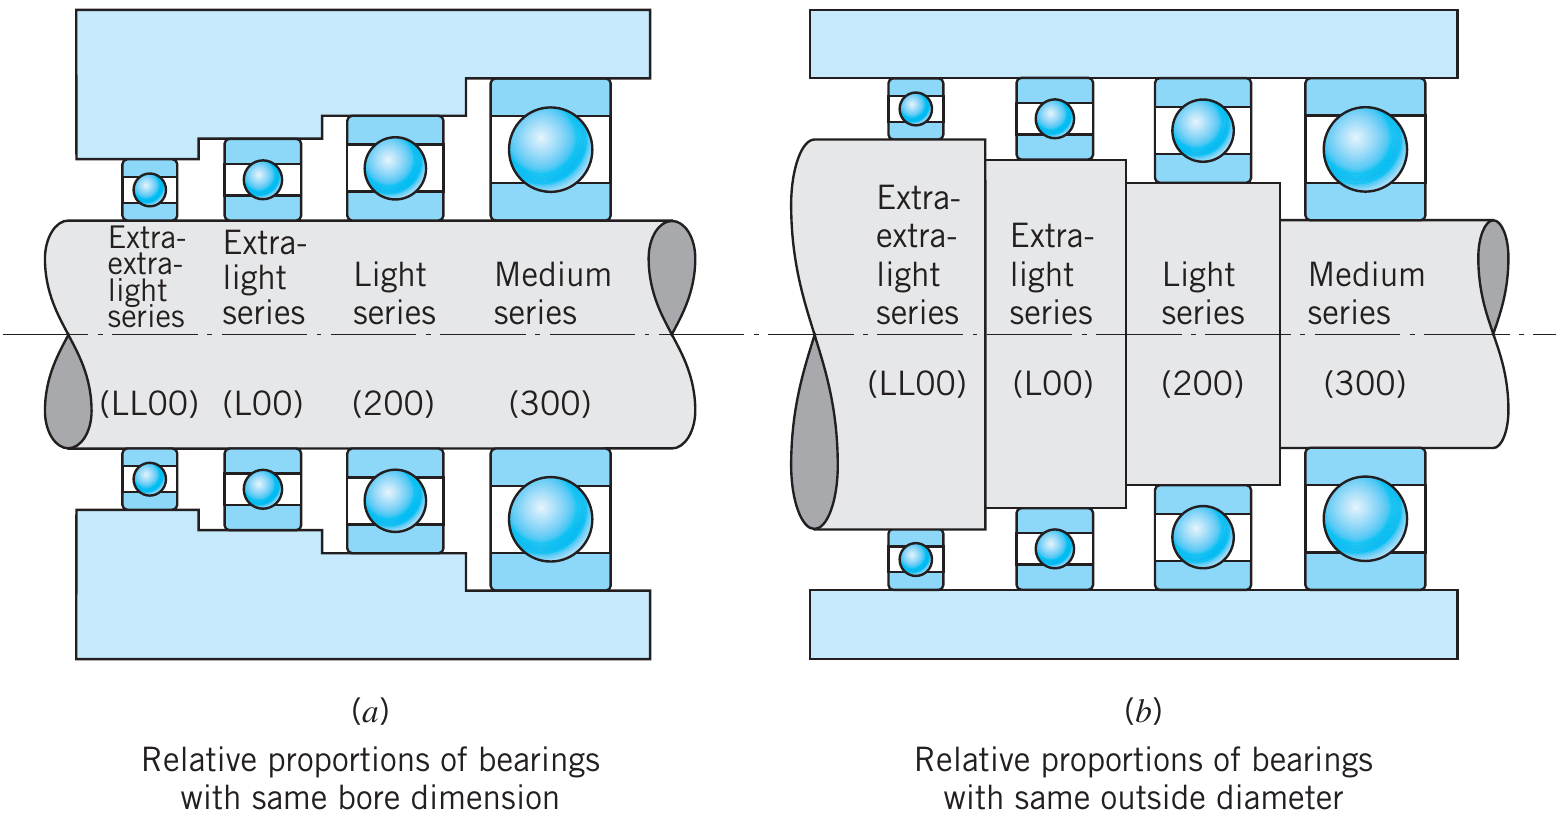
\includegraphics[width=.9\linewidth]{./pictures/bearing-series.png}
\end{center}
\end{frame}

\begin{frame}[label={sec:orgb85b70b}]{Bearing Table}
\begin{center}
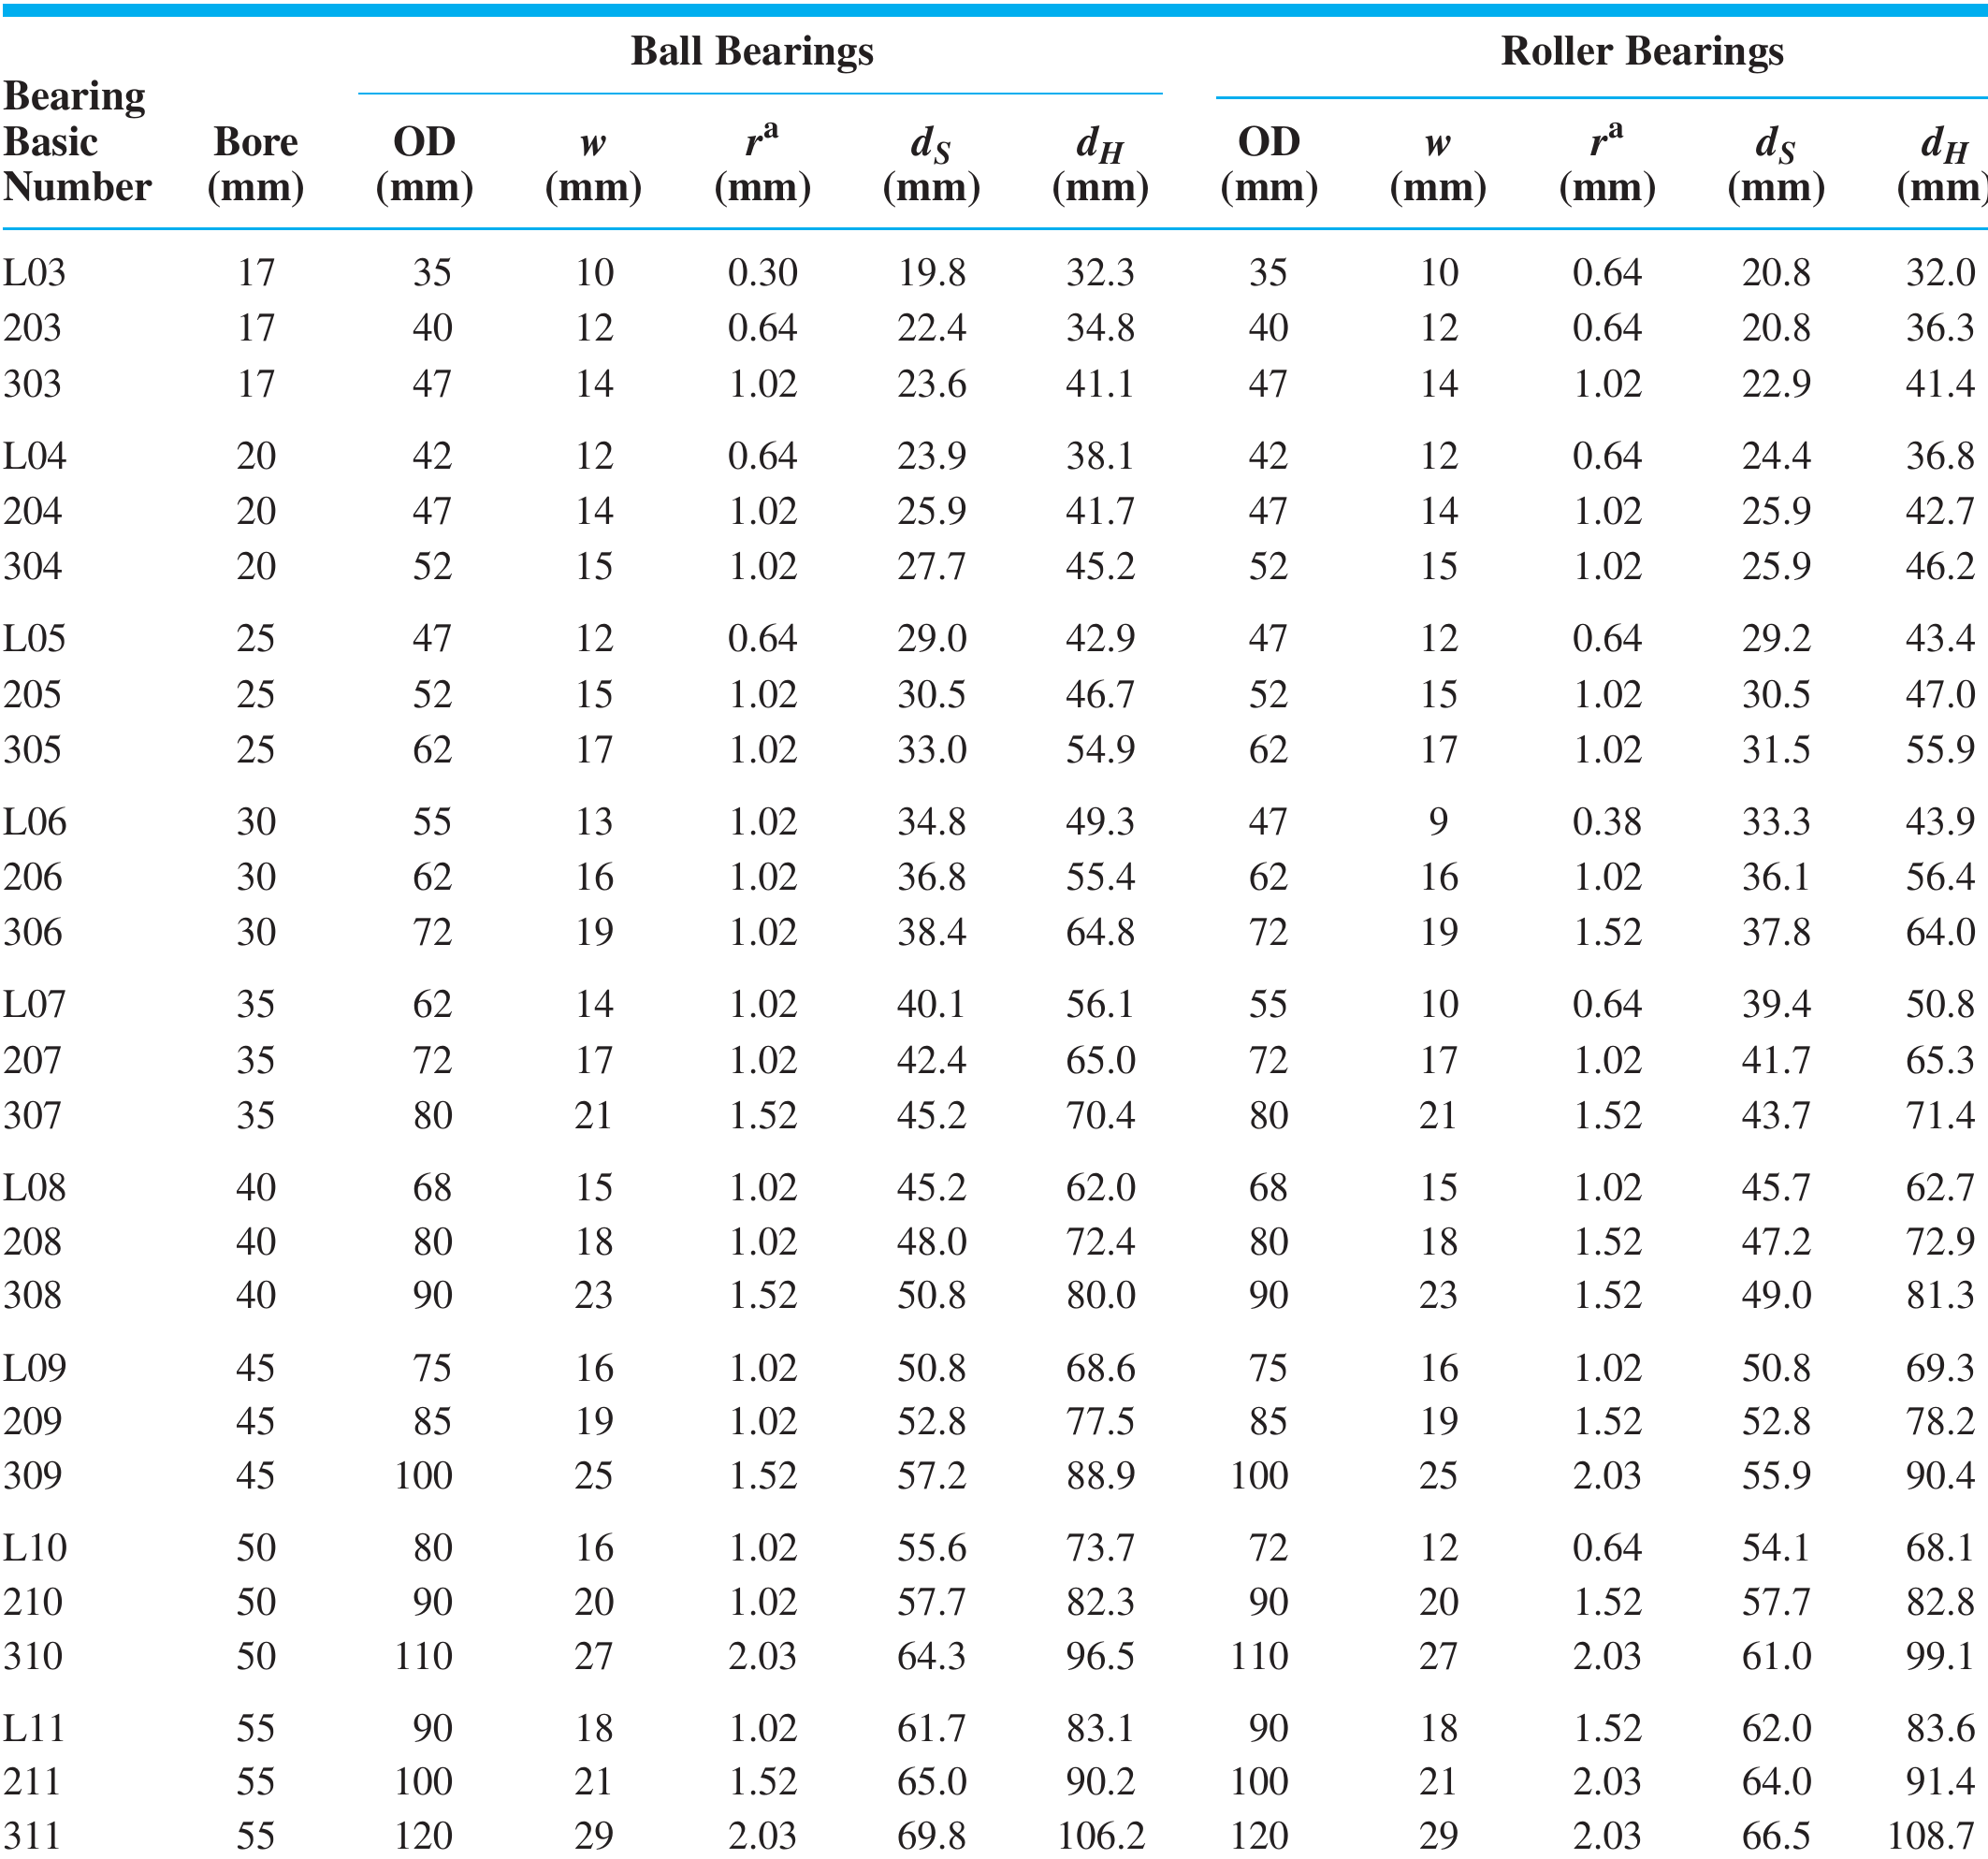
\includegraphics[width=0.8\textwidth]{./pictures/bearing-table.png}
\end{center}
\end{frame}

\begin{frame}[label={sec:orga008984}]{Bearing Life Requirement}
\begin{align*}
    L &= L_R K_r \left( \frac{C}{F_e} \right)^{10/3} \\
    C &= F_e \left( \frac{L}{K_r L_R} \right)^{0.3}
\end{align*}

\begin{center}
\begin{tabular}{ll}
\(L\) & life corresponding to equivalent load \(F_e\)\\\empty
\(L_R\) & life corresponding to rated capacity = 9 \(\times\) 10\(^7\) rev\\\empty
\(K_r\) & reliability factor\\\empty
\(C\) & rated capacity\\\empty
\(F_e\) & equivalent load\\\empty
\end{tabular}
\end{center}
\end{frame}

\begin{frame}[label={sec:org1d31eed}]{Bearing Rated Capacity}
\begin{center}
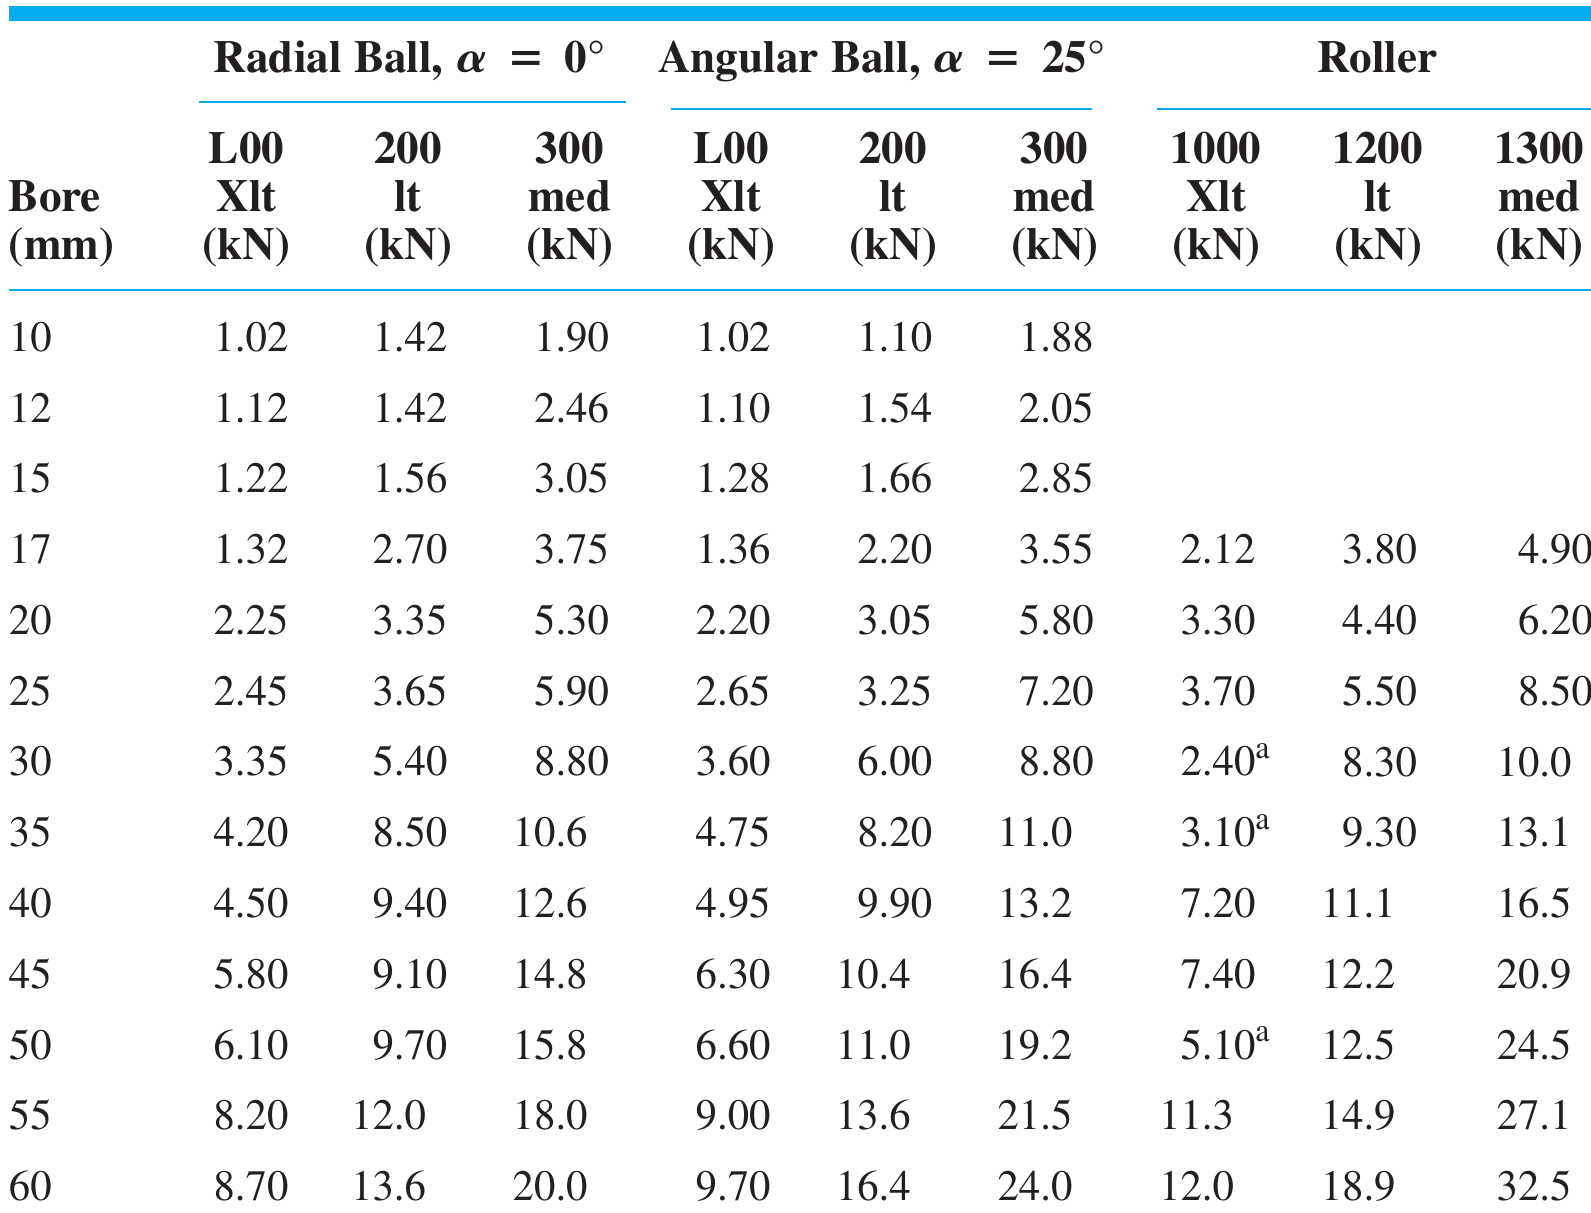
\includegraphics[width=.9\linewidth]{./pictures/bearing-rated-capacity.png}
\end{center}
\end{frame}

\begin{frame}[label={sec:orgebf3b12}]{Reliability Factor}
\begin{center}
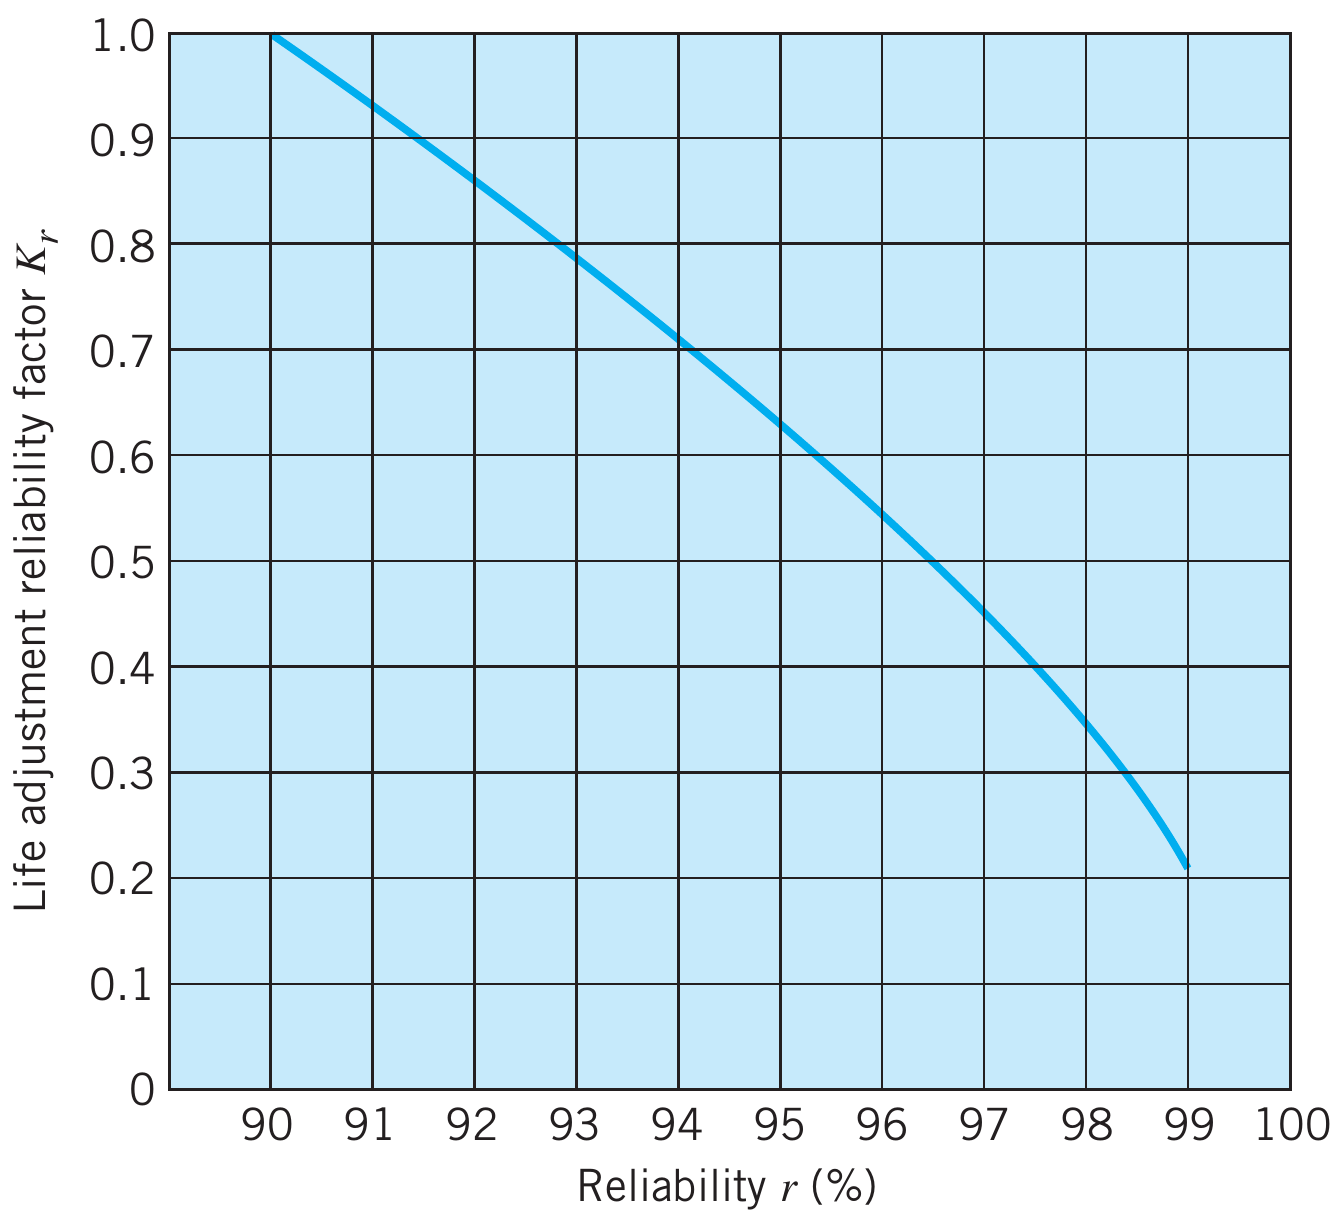
\includegraphics[width=.9\linewidth]{./pictures/reliability-factor.png}
\end{center}
\end{frame}

\begin{frame}[label={sec:orgd365cbb}]{Equivalent Load}
Let \(e = F_a / F_r\)

for radial ball bearings

\begin{align*}
    F_e = \left\{
    \begin{array}{ll}
        F_r & e < 0.35 \\
        F_r \left[ 1 + 1.115(e - 0.35) \right] & 0.35 < e < 10 \\
        1.176 F_a & e > 10
    \end{array}
    \right.
\end{align*}

for angular ball bearings

\begin{align*}
    F_e = \left\{
    \begin{array}{ll}
        F_r & e < 0.68 \\
        F_r \left[ 1 + 0.87(e - 0.68) \right] & 0.68 < e < 10 \\
        0.911 F_a & e > 10
    \end{array}
    \right.
\end{align*}
\end{frame}

\begin{frame}[label={sec:org429df62}]{Typical Bearing Design Life}
\begin{center}
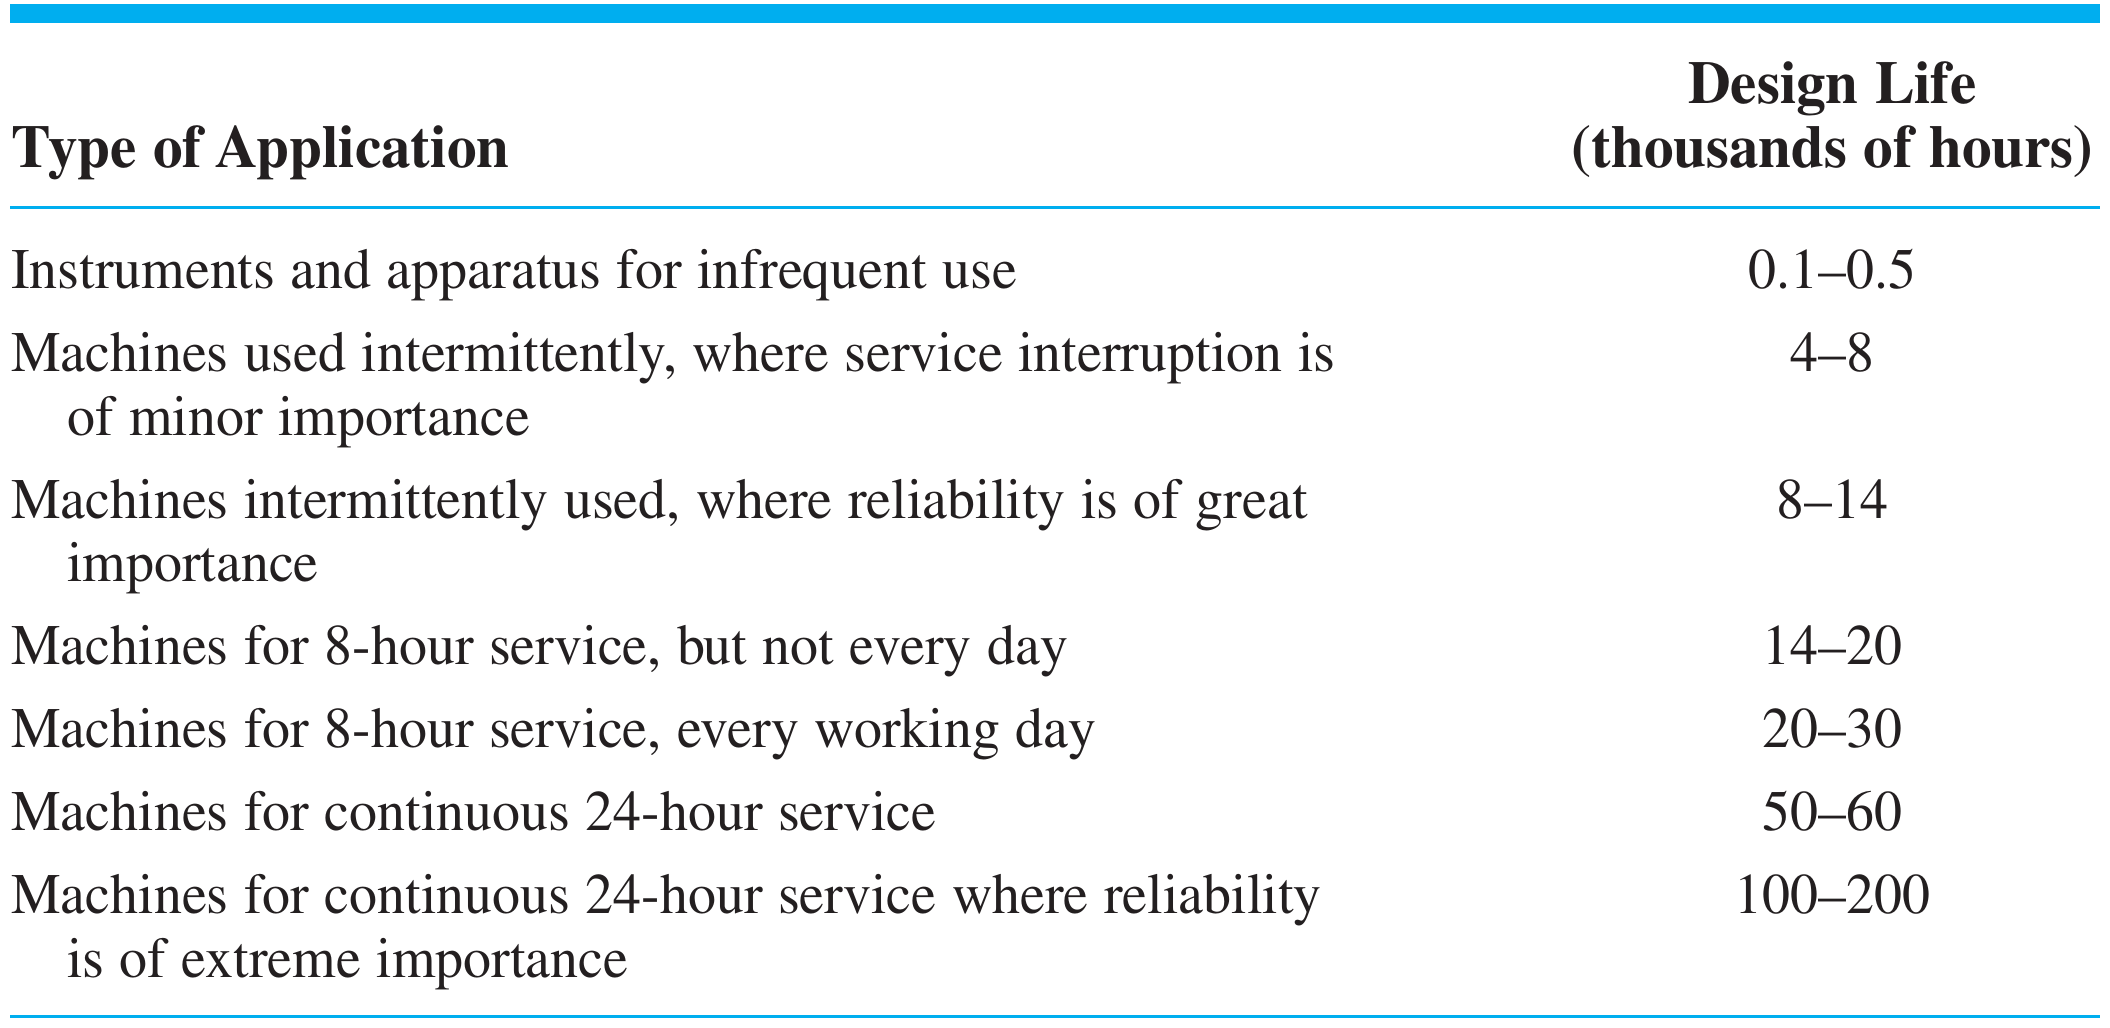
\includegraphics[width=\textwidth]{./pictures/designed-bearing-life.png}
\end{center}
\end{frame}

\begin{frame}[label={sec:org1c7bacc}]{Example}
Select a radial ball bearing for a shaft intended for a continuous 8-hr-a-day operation at 1800 rpm with 95\% reliability. Axial and radial loads are 1.2 kN and 1.5 kN, respectively.
\end{frame}

\begin{frame}[label={sec:orgdee2892}]{Solution}
\begin{itemize}
\item First, we need to calculated \(F_e\).

$$e = \frac{F_a}{F_r} = \frac{1.2}{1.5} = 0.8$$

\item For radial ball bearing,
\end{itemize}

\begin{align*}
    F_e &= 1500 \left[ 1 + 1.115(0.8 - 0.35) \right] \\
        &= 2253 \text{ N}
\end{align*}
\end{frame}

\begin{frame}[label={sec:org80da324}]{Solution}
\begin{itemize}
\item Required life for 8-hr-a-day service (assumed every day) = 30000 hrs

\item Life in revolutions

$$L = 1800(30000)(60) = 3.24 \times 10^9 \text{ revolutions}$$

\item For 95\% reliability \(K_r\) = 0.63
\end{itemize}

\begin{align*}
    C = 2253 \left( \frac{3.24 \times 10^9}{0.63 (9 \times 10^7)} \right)^{0.3} = 7583 \text{ N} = 7.58 \text{ kN}
\end{align*}
\end{frame}

\begin{frame}[label={sec:org1fd64b9}]{Solution}
\begin{itemize}
\item For extra-light, light, and medium series, the required bore are 55, 35, and 30 mm, respectively

\item The models corresponding to the bore are L11, 207, and 306, respectively.
\end{itemize}
\end{frame}
\end{document}